
Este apêndice tem como objetivo registrar os dados obtidos durante a execução dos cenários de teste. Ao longo do apêndice estão presentes
Imagens do processo de auto-localização e do resultado da localização, como pode ser observado a seguir.

\section{Cenário de Teste 1}

Este cenário está dividido em 5 (cinco) exemplos, os quais são apresentados a seguir, contemplando todo o processo de auto-localização
em cada exemplo, a partir da apresentação das Imagens abaixo.

\subsection{Exemplo 1}

\begin{figure}[H]
  \centering
  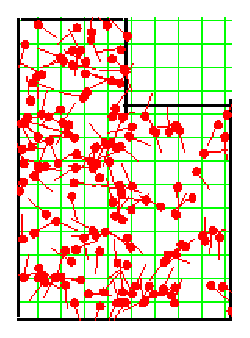
\includegraphics[scale=0.6]{figuras/cen1_ex1/1.eps}
  \caption[Partículas Iniciais]{Partículas iniciais}
  \label{img:cen1_ex1_1}
\end{figure}

\begin{figure}[H]
  \centering
  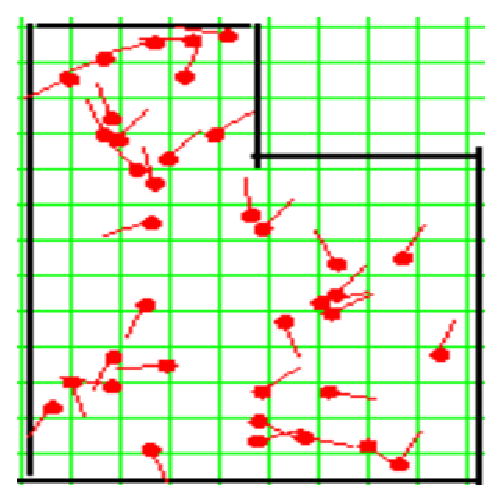
\includegraphics[scale=0.6]{figuras/cen1_ex1/2.eps}
  \caption[Primeiro Ciclo de Filtragem]{Primeiro ciclo de filtragem}
  \label{img:cen1_ex1_2}
\end{figure}

\begin{figure}[H]
  \centering
  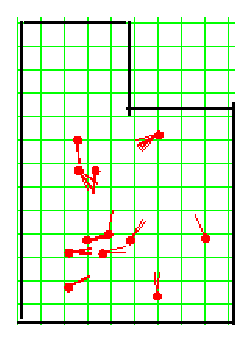
\includegraphics[scale=0.6]{figuras/cen1_ex1/3.eps}
  \caption[Segundo Ciclo de Filtragem]{Segundo ciclo de filtragem}
  \label{img:cen1_ex1_3}
\end{figure}

\begin{figure}[H]
  \centering
  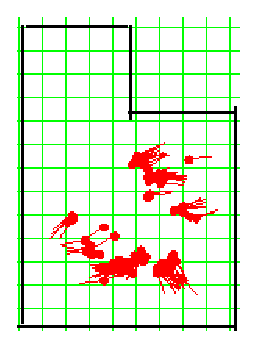
\includegraphics[scale=0.6]{figuras/cen1_ex1/4.eps}
  \caption[Terceiro Ciclo de Filtragem]{Terceiro ciclo de filtragem}
  \label{img:cen1_ex1_4}
\end{figure}

\begin{figure}[H]
  \centering
  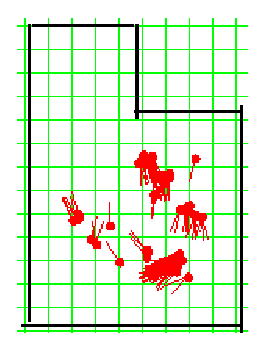
\includegraphics[scale=0.6]{figuras/cen1_ex1/5.eps}
  \caption[Quarto Ciclo de Filtragem]{Quarto ciclo de filtragem}
  \label{img:cen1_ex1_5}
\end{figure}

\begin{figure}[H]
  \centering
  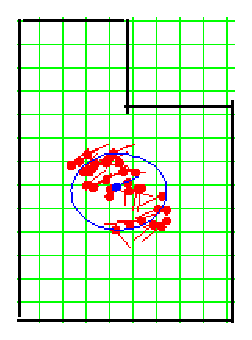
\includegraphics[scale=0.6]{figuras/cen1_ex1/6.eps}
  \caption[Quinto Ciclo de Filtragem]{Quinto ciclo de filtragem}
  \label{img:cen1_ex1_6}
\end{figure}

\begin{figure}[H]
  \centering
  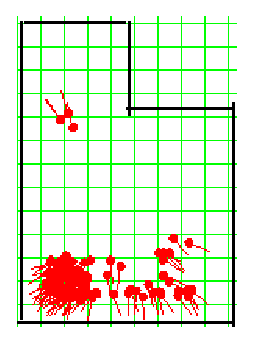
\includegraphics[scale=0.6]{figuras/cen1_ex1/7.eps}
  \caption[Sexto Ciclo de Filtragem]{Sexto ciclo de filtragem}
  \label{img:cen1_ex1_7}
\end{figure}

\begin{figure}[H]
  \centering
  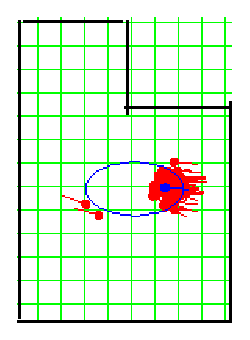
\includegraphics[scale=0.6]{figuras/cen1_ex1/8.eps}
  \caption[Sétimo Ciclo de Filtragem]{Sétimo ciclo de filtragem}
  \label{img:cen1_ex1_8}
\end{figure}

\begin{figure}[H]
  \centering
  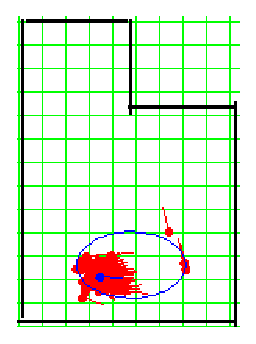
\includegraphics[scale=0.6]{figuras/cen1_ex1/9.eps}
  \caption[Oitavo Ciclo de Filtragem]{Oitavo ciclo de filtragem}
  \label{img:cen1_ex1_9}
\end{figure}

\begin{figure}[H]
  \centering
  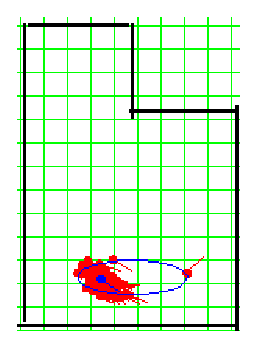
\includegraphics[scale=0.6]{figuras/cen1_ex1/10.eps}
  \caption[Nono Ciclo de Filtragem]{Nono ciclo de filtragem}
  \label{img:cen1_ex1_10}
\end{figure}
